\section{Materials and Methods}

\subsection{Study Site}

Site selection followed a systematic filtering process driven by project requirements and practical constraints. The study was supported by a federal grant that mandated research be conducted on federal lands. We selected Vandenberg Space Force Base (VSFB, 34.7398°N, 120.5725°W) in Santa Barbara County, California, based on several key advantages: mild winters with infrequent frost events, extensive historical plantings of blue gum eucalyptus (\textit{Eucalyptus globulus}) that have created suitable overwintering habitat throughout the installation, and restricted access that provided security for long-term equipment deployment. The military base contains thirty documented monarch overwintering groves, with several sites consistently ranking within the top 10\% of population counts statewide over the past decade \parencite{xercessocietyWesternMonarchButterfly2025}. 

Working with the base's monarch conservation coordinator, we initially screened twelve locations from the thirty sites based on their documented capacity to support monarch aggregations and provide year-round access. This collaboration leveraged local expertise from managing Western Monarch Thanksgiving Count activities for multiple years \parencite{xercessocietyWesternMonarchButterfly2025}. From these twelve candidate sites, we deployed monitoring equipment at ten unique locations across both study seasons: four sites during the 2023-2024 season and ten sites during the 2024-2025 season. However, due to low monarch populations during the 2023-2024 season and no observed overwintering behavior in the 2024-2025 season, only two sites (Spring Canyon and UDMH) produced measurable butterfly clusters suitable for our study.

Spring Canyon (34.6315°N, 120.6182°W) represents the most productive and historically reliable overwintering site on VSFB. Located in South Base within 300 meters of Space Launch Complex 4, this approximately 2.0-hectare site consists entirely of mature blue gum eucalyptus trees reaching heights of approximately 40 meters. An unnamed perennial creek runs through the center of the grove, creating a riparian corridor that supports heterogeneous canopy structure with variable tree spacing and diverse understory vegetation. Surf Road, an infrequently used paved access road, bisects both the perennial creek and forest canopy. 

The second site, UDMH site (34.6719°N, 120.5950°W), also located in South Base, comprises a 5.1-hectare eucalyptus grove planted in windrows adjacent to a waste treatment facility. The uniformly spaced trees maintain a largely clear understory with scattered low shrubs. Although only recently documented as an overwintering location in 2022, UDMH immediately emerged as a significant site, supporting over 6,000 monarchs during its initial 2022 count and ranking among the base's highest population sites.

% [Figure here showing all thirteen groves, with different symbology for the various subsets]

\subsection{Monitoring Strategy}

Equipment deployment strategies differed between monitoring seasons to accommodate research objectives and field experience. During the 2023-2024 season, we employed two strategies: targeted deployments at sites with confirmed monarch presence, and anticipatory deployments at locations where monarchs were expected based on historical data but not currently observed. Targeted deployments concentrated at Spring Canyon and UDMH where active aggregations were documented throughout the season. Anticipatory deployments occurred at four overwintering sites: additional locations within Spring Canyon and UDMH, plus SLC-6 and Tangair. In the 2024-2025 season, no monarchs were recorded at these anticipatory deployment sites; consequently, these data are excluded from analysis.

Building on insights from the 2023-2024 season, for the 2024-2025 season we modified our approach to establish monitoring stations at ten sites before monarch arrival, based on historical occurrence records compiled by the base conservation coordinator. This expanded spatial coverage aimed to capture greater environmental variation across potential overwintering sites. However, the 2024-2025 season coincided with historically low monarch abundance throughout California \parencite{xercessocietyWesternMonarchButterfly2025}, resulting in no observed clustering behavior at any of the ten monitored locations. Consequently, our analysis focuses exclusively on data collected during the 2023-2024 season.

\subsection{Field Equipment}

To observe changes in monarch abundance in response to strong wind events, we deployed remote monitoring equipment near butterfly clusters at overwintering sites. Field observations utilized 15-meter telescoping fiberglass poles (Max-Gain Systems, Inc., Marietta, GA) anchored at three points using ground anchors with guy lines securing both the top and base to create stable, freestanding structures. 

Poles were positioned 4-17 meters from cluster locations. This range, determined through field testing, balanced image resolution requirements for our grid-based counting method against disturbance minimization. Closer positioning compromised field of view, while greater distances degraded butterfly visibility below classification thresholds. Pole placement considered ground stability for the 15-meter structures, infrastructure clearance requirements, and clear viewing angles. When deploying near active clusters, we approached from directions that minimized disturbance; no butterfly dispersal was observed during equipment deployment. 

We monitored monarch abundance using modified trail cameras (GardePro E7 and E8, Shenzhen, China) configured for near-infrared imaging to enhance contrast between clustering butterflies and surrounding vegetation. Trail cameras were selected for their durability for extended field deployment, native time-lapse functionality, and modification potential. Near-infrared wavelength selection followed previous literature demonstrating effectiveness for butterfly population estimation \parencite{hristovEstimatingOverwinteringMonarch2019}. 

Hardware modifications exploited the camera's internal filter-switching mechanism by engaging nighttime mode to access the clear glass filter position, then disconnecting power to prevent reversion to the infrared cut filter. Near-infrared pass filters (>850 nm) were mounted externally to restrict incoming light to NIR wavelengths. This configuration produced images where clustering butterflies appeared as dark masses against bright eucalyptus foliage reflectance in the near-infrared spectrum. Field validation confirmed sufficient contrast for visual distinction of monarch clusters from background vegetation, supporting our human-labeler analytical approach.

Cameras were mounted atop poles using lightweight tie-down straps and positioned horizontally toward butterfly clusters at roosting height. The wireless live view feature enabled real-time preview and precise camera aiming during deployment. Cameras operated in time-lapse mode with motion detection disabled. 

Sampling interval selection balanced temporal resolution, battery life, and data processing feasibility through empirical optimization and rigorous statistical validation. Initial deployments used 10-minute intervals to capture significant changes in butterfly abundance, which preliminary observations indicated occurred on hourly rather than minute scales, while maintaining approximately 6-week continuous operation. Post-deployment statistical analysis using mixed-effects models and information-theoretic approaches systematically compared multiple sampling intervals across deployments. We conducted sequential subsample analyses starting with full temporal resolution and progressively testing reduced frequencies. Information-theoretic model comparison using Akaike Information Criterion (AIC) demonstrated that 30-minute intervals provided optimal balance, losing less than 5\% of information compared to full temporal resolution (measured by root mean square error) while reducing image classification workload by 67\%. Variance comparison analysis and visual assessment of fitted trend lines confirmed that this interval preserved essential time-series patterns including diurnal activity cycles, weather-response dynamics, and multi-day population trends. Battery life constraints and field deployment logistics further supported this interval choice, enabling extended autonomous operation essential for capturing complete behavioral sequences during variable weather conditions.

To quantify the wind conditions hypothesized to influence butterfly behavior, wind monitoring equipment consisted of Rain Wise WindLog Wind Data Loggers (Rain Wise Inc., Trenton, Maine) installed at pole apices to measure wind at heights approximating butterfly roosting locations. These instruments recorded average wind speed and maximum wind gust at one-minute intervals, the highest frequency supported by the sensors. This recording interval enabled calculation of wind speed variance within each photographic sampling period, capturing gustiness lost with longer averaging periods. 

To systematically organize our heterogeneous monitoring efforts, we defined discrete monitoring periods as deployment units. Each deployment represented a unique combination of monitoring location, camera configuration (including camera ID, mounting height, and viewing angle), associated wind measurements, and temporal coverage period. Since equipment was frequently reused across locations and time periods, this deployment-based structure provided standardized sampling units that accounted for variation in environmental conditions and equipment configurations while treating each deployment as independent for statistical analyses. This approach produced time-series images from each deployment for estimating monarch cluster abundance through systematic grid-based counting methods, enabling analysis of abundance patterns in relation to wind speed and other environmental variables.

% [A tree with a measuring device and a diagram AI-generated content may be incorrect.]

\subsection{Image Analysis}

\subsubsection{Grid-based Counting Method}

To quantify changes in monarch butterfly abundance from collected imagery, we developed a systematic grid-based counting protocol balancing accuracy with the practical constraints of analyzing tens of thousands of images. This approach addressed the challenge of estimating abundance in large aggregations where individual counts would be prohibitively time-consuming and emulated field researcher methods, including those used in the annual Thanksgiving Count \parencite{xercessocietyManagingMonarchsWest2018}. We subdivided each image using a grid overlay system where human labelers assigned order-of-magnitude estimates per cell. Grid dimensions remained fixed throughout each deployment to ensure consistency. Custom software developed using the Electron framework in JavaScript facilitated this labeling effort.

Grid cell size varied by deployment based on camera-to-cluster distance. Cell dimensions were optimized to ensure most occupied cells contained butterflies in the 10–99 count range, balancing classification efficiency with spatial resolution. This standardization minimized cells alternating between widely different order-of-magnitude categories across the time series.

\subsubsection{Counting Protocol}

Human labelers estimated butterfly abundance within each grid cell using four order-of-magnitude categories: 0 (no butterflies), 1–9 (single digits), 10–99 (dozens), and 100–999 (hundreds). Labelers trained using a comprehensive online guide with example images and detailed classification criteria (\url{https://kylenessen.github.io/monarch_trailcam_classifier/}). The protocol prioritized efficiency while maintaining consistency across observers.

Because abundance estimates derived exclusively from two-dimensional photographic images, our classification protocol quantified only butterflies visible in the image plane without estimating three-dimensional cluster structure or depth. This approach intentionally excluded hidden individuals behind visible butterflies in overlapping aggregations, providing a conservative but consistent measure reflecting observable surface area rather than total volume. For cells containing partial butterflies at grid boundaries, labelers included these in counts unless double-counting would cause an adjacent cell to move to a higher category. When butterfly counts fluctuated between categories across the time series, we consistently applied the lower estimate to maintain conservative abundance estimates.

In addition to estimating monarch abundance, labelers recorded whether cells received direct sunlight. Direct sunlight classification presented challenges because oversaturated conditions eliminated the contrast enabling butterfly detection in shaded areas. Labelers classified cells as receiving direct sunlight when branches or butterflies exhibited additional illumination clearly from direct rather than indirect light, even when individual butterflies became difficult to distinguish due to pixel oversaturation. This classification required careful attention to subtle shape recognition and contextual awareness about butterfly locations established from previous images in the time series. This measurement was recorded only for occupied cells and stored separately.

Labelers received ongoing feedback throughout the classification process. All classifications underwent review for common errors including mislabeled cells, incorrect category assignments, and inconsistent counting criteria application. Direct communication of corrections to labelers ensured consistent protocol application.

\subsubsection{Abundance Calculation}

We calculated an abundance index for each frame by summing the products of cell counts and their assigned category values across all grid cells, employing conservative estimates using minimum values within each order-of-magnitude category:

\begin{equation}
\text{Abundance index} = \sum_{i} \rho_i \times C_i
\end{equation}

where $\rho_i$ represents the number of cells in category $i$, and $C_i$ represents the conservative estimate for that category. We used minimum category values ($C_1 = 1$ for category 1–9, $C_2 = 10$ for category 10–99, and $C_3 = 100$ for category 100–999) rather than midpoint or maximum values to ensure temporal analyses reflected genuine population shifts rather than estimation uncertainty.

\subsection{Temperature Data Extraction}

Temperature represents a critical environmental variable influencing monarch activity patterns and potentially confounding wind effects. Ambient temperature data were extracted from trail camera images using optical character recognition (OCR). Each camera displayed temperature readings on the image overlay, but these values were not accessible through EXIF metadata, necessitating visual extraction methods. We developed an automated Python script utilizing OCR technology to extract temperature values from approximately 56,000 images across all deployments. The extraction process employed multiple preprocessing strategies and pattern matching algorithms to accommodate variations in image quality and display characteristics.

Following initial automated extraction, we manually reviewed and corrected edge cases where OCR failed or produced anomalous values. All temperature data underwent systematic quality control through visualization of deployment-specific time series, enabling identification and correction of erroneous values. This process ensured complete temperature coverage for all analyzed images, providing the ambient temperature covariate required for our statistical models.

\subsection{Statistical Analysis}
\label{sec:statistical-analysis}

\subsubsection{Data Preparation}

Statistical analysis employed a lag-based framework to capture the temporal dynamics of butterfly responses to environmental changes, comparing butterfly counts between consecutive 30-minute intervals. Observation pairs were constructed by matching counts at time $t$ with counts at time $t-30$ minutes, applying a ±5 minute tolerance window to accommodate minor temporal variations in image capture. The response variable (change in butterfly abundance between time points) underwent cube root transformation to achieve approximate normality while preserving directional information: $y = \text{sign}(\Delta) \times |\Delta|^{1/3}$, where $\Delta$ represents the difference in butterfly counts. While exploratory data analysis revealed generally well-behaved distributions, we observed bimodality in the raw butterfly abundance data driven primarily by a single anomalous event at deployment SC8. At this deployment, a large butterfly aggregation abruptly declined to near zero without corresponding changes in the measured environmental variables (wind speed, temperature, or solar exposure). This singular event was unlike any other observation in the dataset. We retained this deployment in the final analysis for two reasons: first, to maximize sample size and avoid arbitrary data exclusion, and second, sensitivity analysis showed that the cube root transformation of abundance differences adequately addressed the distributional concerns, with model selection and parameter estimates remaining consistent whether SC8 was included or excluded. The transformation approach made the anomaly's inclusion or exclusion immaterial to the final results. Observation pairs where both time points recorded zero butterflies were excluded as uninformative, reducing the dataset from approximately 2,500 potential pairs to 1,894 analyzable observations across 115 unique deployment-day combinations.

\subsubsection{Variable Selection}

Predictor variables were selected to test specific hypotheses while avoiding multicollinearity. Maximum wind gust speed during each 30-minute interval served as the primary wind metric, with alternative wind measurements (average sustained speed, modal gust, gust standard deviation) excluded due to high correlation ($r > 0.75$). Environmental predictors included average temperature between observation pairs, number of butterflies in direct sunlight at the previous time point, and minutes elapsed since the first observation of each day to capture diurnal patterns. Total butterfly count at the previous time point was included as a control variable, enabling distinction between proportional and absolute changes in abundance. When included, this variable tests effects on proportional change; when excluded, models test effects on absolute change.

\subsubsection{Model Framework}

Analysis employed generalized additive mixed models (GAMMs) implemented through the mgcv package in R. Model selection followed an information-theoretic approach, comparing 48 candidate models using Akaike Information Criterion (AIC). The candidate set comprised two fundamental frameworks: models including the lag abundance term (24 models) and models excluding it (24 models), with each framework containing null models, single predictor models, additive combinations, two- and three-way interactions, and models incorporating smooth terms for non-linear relationships. Random effects structure accounted for variation at three hierarchical levels: deployment location, observer, and deployment-day. Temporal autocorrelation within days was addressed using a first-order autoregressive (AR1) correlation structure grouped by deployment-day. All models were fitted using restricted maximum likelihood (REML) estimation.

To test specifically for threshold effects at the proposed 2 m/s disruptive wind speed, we conducted a threshold wind disruption analysis using an alternative wind metric. We repeated the entire model selection process, replacing maximum wind gust speed with a threshold-based predictor: the count of minutes within each 30-minute observation period where wind gusts equaled or exceeded 2 m/s. This variable ranged from 0 to 30 minutes and was tested using the same 48 model structures, allowing direct comparison of continuous versus threshold-based wind effects.

\subsubsection{Model Validation}

Model assumptions were verified through standard residual diagnostics including examination of residual distributions, fitted versus residual plots, and quantile-quantile plots. Convergence was confirmed for all candidate models in both the primary and threshold wind disruption analyses. Model performance and predictor significance were evaluated through AIC comparison, with models differing by less than 2 AIC units considered equivalent.

\subsubsection{Statistical Power Analysis}

To evaluate whether our study had adequate statistical power to detect wind effects if present, we conducted a simulation-based power analysis. This approach assessed our ability to detect various effect sizes given our sample size of 1,894 paired observations. We simulated 200 datasets from the best-fitting model (which excluded wind effects) and artificially introduced wind effects of known magnitude ranging from 0.05 to 0.20 standard deviations of the response variable. For each effect size, we refitted models including wind terms to determine the proportion of simulations where the artificial effect was detected as statistically significant ($\alpha = 0.05$). This simulation approach accounts for the complexity of our GAMM framework and hierarchical data structure, providing robust estimates of statistical power for detecting wind effects across a range of biologically plausible magnitudes.

\subsubsection{Dynamic Window Analysis}

To examine whether day-to-day changes in roost size depend on cumulative weather exposure aligned with butterfly roosting biology, we conducted a complementary analysis using dynamic temporal windows. This approach tested wind effects at a daily scale, capturing overnight and full-day weather exposure that the 30-minute lag analysis could not assess.

We constructed two window definitions to test the robustness of our findings. The sunset window spanned from the previous day's maximum butterfly count to the current day's last observation, approximating functional sunset when roosting decisions finalize. This biologically-aligned window varied in duration (mean = 29.6 hours) to capture the complete exposure period from peak aggregation through the subsequent roosting decision point. The 24-hour window provided a standardized comparison, extending exactly 24 hours from the previous day's maximum count.

Daily aggregates were computed for each deployment-day combination, including maximum butterfly count, 95th percentile count, and mean of the top three counts. We retained only days with 15-25 daytime photographs to ensure adequate temporal coverage, then constructed consecutive day pairs separated by exactly one day. Pairs where both days recorded zero butterflies were excluded as uninformative. The response variable, defined as the change in maximum daily count between consecutive days, underwent signed square root transformation to achieve approximate normality while preserving directional information.

Weather metrics were calculated within each dynamic window. Temperature variables included minimum, maximum, and mean values, plus cumulative metrics such as degree-hours above 15°C. Wind measurements comprised average sustained speed, maximum gust, cumulative gust exposure, and time above the proposed 2 m/s threshold. Direct sun exposure was quantified as the cumulative count of butterflies observed in direct sunlight across all frames within the window, integrating both exposure duration and instantaneous abundance. We required 95\% data completeness across temperature, wind, and daylight observations, calculated as the geometric mean of coverage ratios.

Variable selection for the dynamic window analysis began with 19 candidate predictors spanning baseline abundance metrics, temperature summaries, wind exposure measures, and cumulative sun exposure. We conducted correlation analysis to identify multicollinearity within predictor families, particularly among the highly intercorrelated wind metrics (all pairwise correlations $r > 0.75$) and temperature variables. Based on this analysis, we selected predictors that minimized redundancy while maintaining interpretability and adequate degrees of freedom relative to sample size.

For wind exposure, we selected maximum wind gust as the primary metric because it captured the variance of all wind variables in a single interpretable measure, showed high correlation with sustained speed, gust summation, and threshold exceedance metrics, and maintained consistency with the 30-minute analysis. We excluded wind mode gust despite its biological relevance because it contained only approximately five unique values across the dataset, causing model convergence issues. Temperature representation focused on non-overlapping summaries that captured both the exposure range (minimum and maximum) and the thermal state at the previous day's peak abundance. We excluded highly correlated metrics such as mean temperature and degree-hours above 15°C to reduce multicollinearity. The cumulative direct sun exposure variable was retained as a biologically relevant measure of thermal conditions that integrated both exposure duration and instantaneous abundance. For the sunset window analysis, we included lag duration (hours) as a control variable to account for varying window lengths.

Model selection followed the same information-theoretic approach as the 30-minute analysis. We evaluated 76 candidate models per window type using generalized additive mixed models with deployment random intercepts and AR(1) temporal correlation structures. The candidate set included null models, single predictors, additive combinations, and models with smooth interaction terms. To address potential overfitting given the reduced sample size (n = 94-96 pairs), we applied conservative thresholds for the ratio of effective degrees of freedom to sample size and conducted leave-one-deployment-out cross-validation on top-performing models. The final predictor set comprised: temperature minimum and maximum, maximum wind gust, cumulative direct sun exposure, and baseline abundance controls.

\begin{figure}[ht]
    \centering
    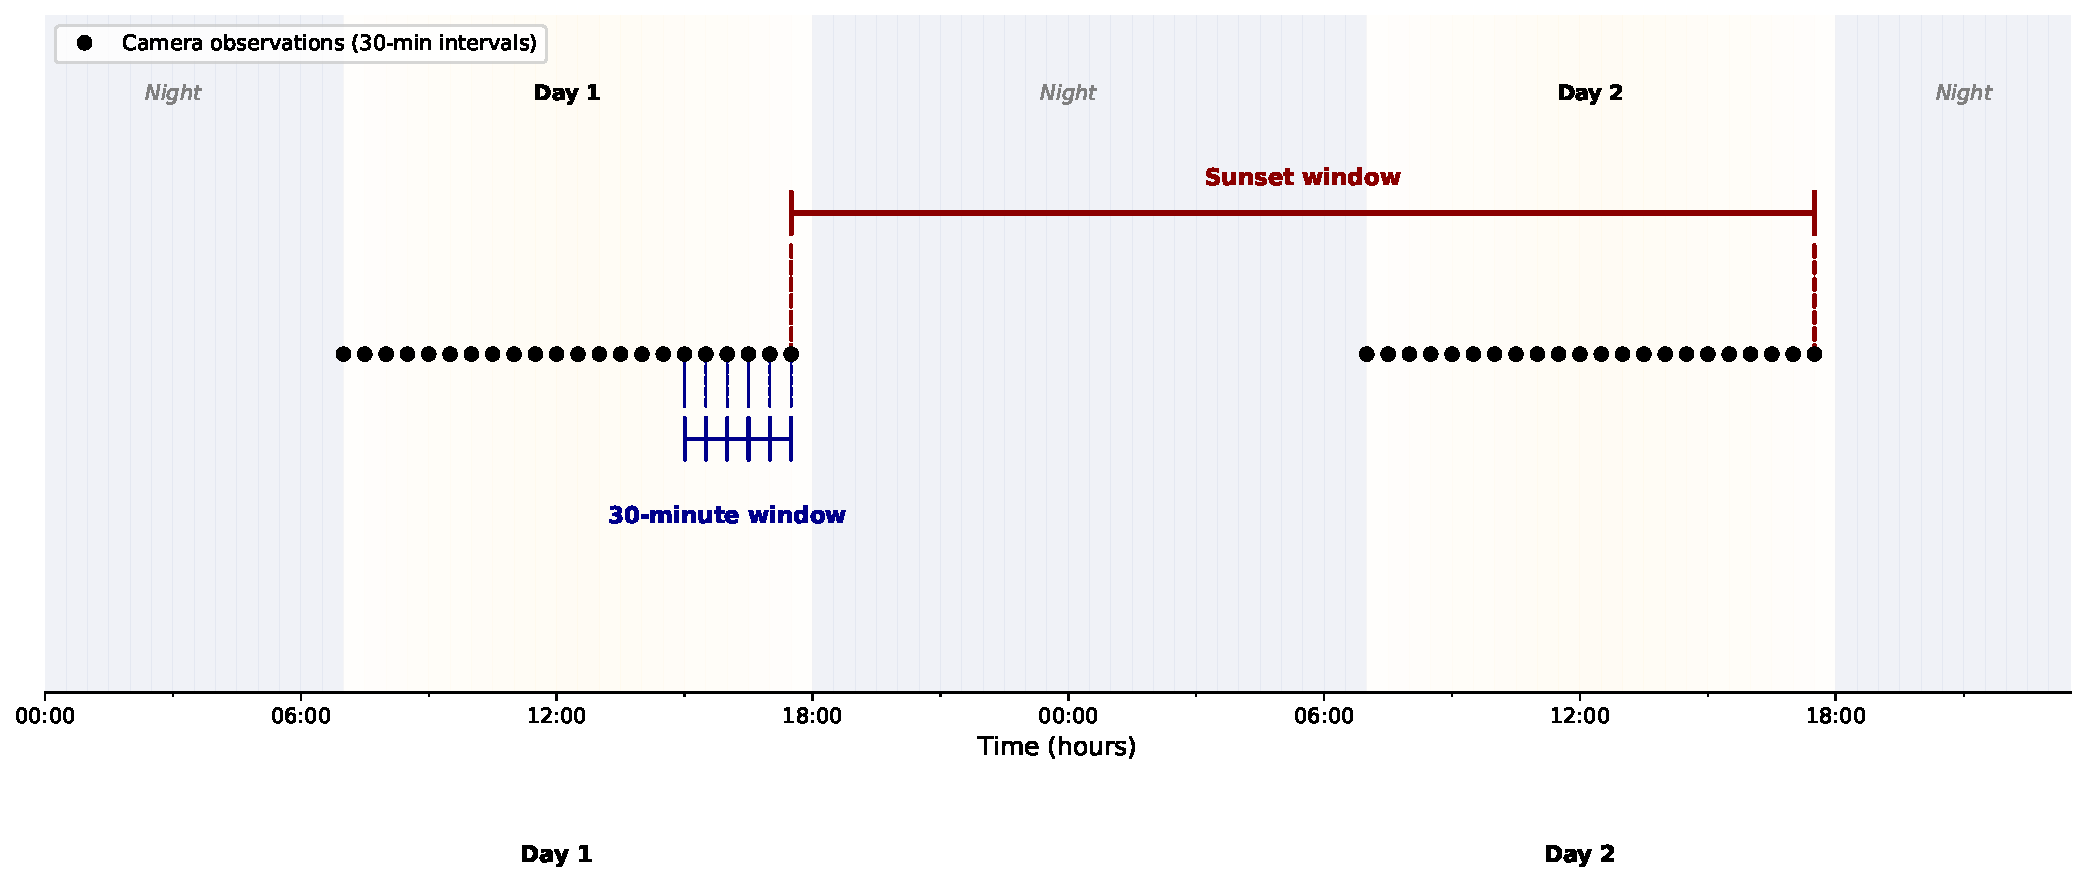
\includegraphics[width=\textwidth]{figures/methods/temporal_windows.pdf}
    \caption{Temporal analysis windows for monarch butterfly monitoring. The figure illustrates two complementary approaches: (1) 30-minute lag analysis comparing consecutive observation intervals to capture immediate responses to environmental changes, and (2) sunset window analysis spanning from the previous day's maximum butterfly count to the current day's final observation (mean duration $\sim$29.6 hours). Camera observations occur at 30-minute intervals during daylight hours only. Background shading indicates day-night cycles with transitions at sunrise and sunset.}
    \label{fig:temporal-windows}
\end{figure}

